\documentclass[11pt,a4paper]{article}
\usepackage[utf8]{inputenc}
\usepackage{geometry}
\usepackage{float}
\usepackage{wrapfig}
\geometry{top=1in, bottom=1in, left=1in, right=1in}

% Mathematics Packages
\usepackage{amsmath}
\usepackage{amssymb}
\usepackage{amsfonts}

% Graphics & Formatting
\usepackage{graphicx}
\usepackage{booktabs}
\usepackage{xcolor}
\usepackage[colorlinks=true, linkcolor=blue, urlcolor=blue, citecolor=blue]{hyperref}

\title{\textbf{Relativistic Invariant Mass Reconstruction in Dimuon Systems via Graph Neural Networks: A Comprehensive Technical Report}}
\author{\textbf{Dataset:} CERN Open Data (2011 SingleMu Primary Dataset, 83,761 Events)}
\date{\number\year-\number\month-\number\day}

\begin{document}

\pagestyle{empty}


\maketitle
\thispagestyle{empty}
\begin{abstract}
This report presents a structured analysis of a machine learning workflow tailored for the reconstruction of the invariant mass spectrum ($M$) in dimuon ($\mu^+\mu^-$) final states. Utilizing 83,761 events extracted from the 2011 CMS Open Data SingleMu primary dataset, we document the data-preprocessing, domain-specific feature engineering, multi-stage partitioning, and the design of an edge-conditioned Graph Neural Network (GNN). Our network accurately maps raw detector kinematics to invariant masses across three orders of magnitude ($0.3\text{ GeV}/c^2$ to $300\text{ GeV}/c^2$), bypassing manual four-vector computation while achieving a log-space $R^2$ score of $0.9915$ and a physical mass resolution ($\sigma_M/M$) of $0.2100$.
\end{abstract}

\hrule
\vspace{0.5cm}

\section{Experimental Context \& Dataset Characterization}

\subsection{Dataset Origin and Purpose}

The dataset originates from the Compact Muon Solenoid (CMS) experiment at the Large Hadron Collider (LHC), specifically derived from the \textbf{2011 SingleMu primary dataset} containing approximately 83k events. This dataset targets high-energy physics (HEP) phenomena where a high-transverse-momentum ($\text{p}_T$) muon triggers the data acquisition system.

The ultimate goal of analyzing dimuon final states is to probe the standard model electroweak sector and search for new physics by reconstructing parent particles. In this specific data slice, the events are filtered to ensure two reconstructed muons are present, allowing the observation of clear resonance peaks ($\omega/\rho$, $\phi$, $J/\psi$, $\psi(2S)$, $\Upsilon$, and the $Z$ boson) spanning a highly non-linear, broad energy spectrum.

\subsection{Raw Feature Dimensionality}

The dataset consists of 21 initial columns. The features per event are organized as follows:
\begin{itemize}
    \item \textbf{Metadata:} \texttt{Run}, \texttt{Event} (unique identifier identifiers).
    \item \textbf{Global/Tracker Flag (\texttt{type1}, \texttt{type2}):} Categorical flags indicating whether a muon is reconstructed as a Global Muon (\texttt{G}, combining tracker and muon spectrometer data) or a Tracker Muon (\texttt{T}, matching inner tracks to isolated segments in the spectrometer).
    \item \textbf{Charge (\texttt{Q1}, \texttt{Q2}):} Discrete values ($\pm 1$) indicating the curvature direction of the track in the $3.8\text{ Tesla}$ solenoid magnetic field.
    \item \textbf{Kinematic Parameters:} Transverse momentum ($p_T$), pseudorapidity ($\eta$), azimuthal angle ($\phi$), total energy ($E$), and the cartesian momentum components ($p_x, p_y, p_z$) for both particles (labeled 1 and 2).
    \item \textbf{Target:} \texttt{M} ($GeV/c^2$), representing the analytically derived invariant mass.
\end{itemize}

\section{Data Preprocessing and Feature Engineering}

\subsection{Preprocessing and Cleaning}

\begin{enumerate}
    \item \textbf{Metadata Deletion:} The columns \texttt{Run} and \texttt{Event} are dropped to prevent the model from memorizing temporal run variations or arbitrary index counters.
    \item \textbf{Duplicate and Missing Values Handling:} Duplicate entries are pruned. Null or missing values are filled using the column median to maintain stability against accidental detector noise without introducing severe statistical bias.
    \item \textbf{Categorical Mapping:} The muon types are converted into numerical flags:
    \begin{equation}
    \text{type} \longrightarrow \begin{cases} 1 & \text{if } \text{Global ('G')} \\ 0 & \text{if } \text{Tracker ('T')} \\ -1 & \text{if } \text{Missing} \end{cases}
    \end{equation}
\end{enumerate}

\subsection{Domain-Specific Feature Engineering}

To maximize the inductive bias of our models, we extract physical relationship indicators between the two particles:
\begin{itemize}
    \item \textbf{Spatial Separation ($\Delta R$):} Measures the angular distance in $\eta$-$\phi$ space.
    \begin{equation}
    \Delta \eta = \eta_1 - \eta_2
    \end{equation}
    \begin{equation}
    \Delta \phi = \text{atan2}(\sin(\phi_1 - \phi_2), \cos(\phi_1 - \phi_2))
    \end{equation}
    \begin{equation}
    \Delta R = \sqrt{(\Delta \eta)^2 + (\Delta \phi)^2}
    \end{equation}
\end{itemize}

\begin{figure}[htbp]
    \centering
    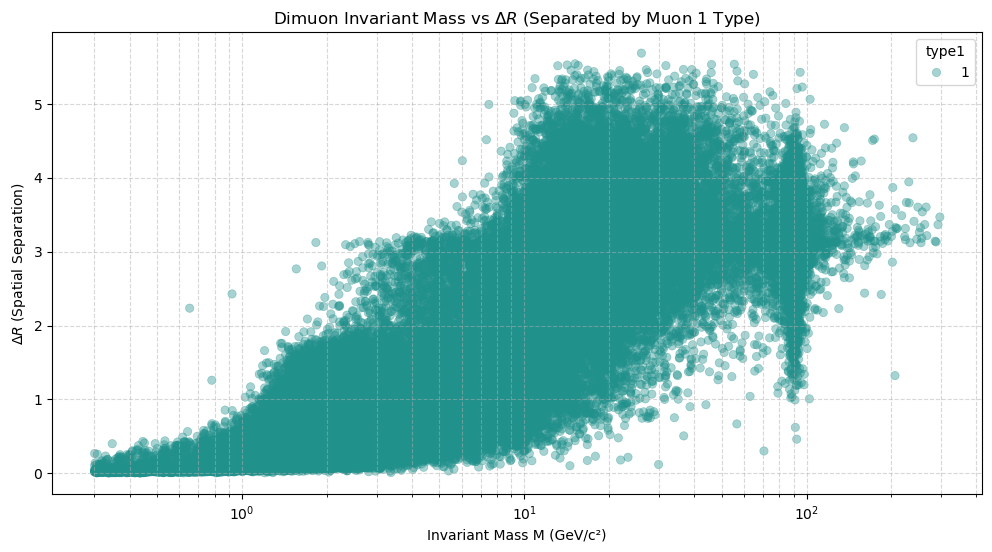
\includegraphics[width=0.75\textwidth]{Dimuon_Invariant_Mass_vs_R.png}
    \caption{Dimuon Invariant Mass vs. $\Delta R$ (Separated by Muon 1 Type). This scatter plot maps the angular distance ($\Delta R$) of the decay products against the system's invariant mass, color-coded by the reconstruction category of the leading muon. The visualization isolates distinct physical resonance bands, illustrating how highly collimated, low-$\Delta R$ states dominate the high-mass electroweak scale while lighter vector mesons exhibit broader angular dispersion.}
    \label{fig:mass_vs_delta_r}
\end{figure}

\begin{itemize}
    \item \textbf{Kinematic Ratios and Summaries:}
    \begin{equation}
    p_{T,\text{ratio}} = \frac{p_{T,1}}{p_{T,2} + 10^{-5}}
    \end{equation}
    \begin{equation}
    p_{T,\text{sum}} = p_{T,1} + p_{T,2}
    \end{equation}
    
    \item \textbf{Conserved Vector Totals:}
    \begin{equation}
    E_{\text{total}} = E_1 + E_2, \quad p_{x,\text{total}} = p_{x,1} + p_{x,2}
    \end{equation}
    \begin{equation}
    p_{y,\text{total}} = p_{y,1} + p_{y,2}, \quad p_{z,\text{total}} = p_{z,1} + p_{z,2}
    \end{equation}
\end{itemize}

\section{Statistical Data Partitioning and Scaling}

\subsection{Three-Way Data Splitting}

To prevent data leakage and evaluate generalization boundaries strictly, the 83k event matrix is divided using a sequential split strategy:
\begin{itemize}
    \item \textbf{Initial Split:} $85\%$ Train-Validation set, $15\%$ Test set.
    \item \textbf{Secondary Split:} The Train-Validation subset is partitioned using a ratio of $17.65\%$ validation, yielding an exact global distribution of \textbf{$70\%$ Training}, \textbf{$15\%$ Validation}, and \textbf{$15\%$ Testing}.
\end{itemize}

\subsection{Asymmetric Feature Scaling Strategy}

Applying a single scaling operation uniformly across categorical labels and skewed kinematics causes severe gradient updates or information loss. We applied a hybrid strategy:
\begin{enumerate}
    \item \textbf{Discrete Features (\texttt{type}, \texttt{Q}):} Left unscaled to preserve their discrete value bounds ($\pm 1$, $0$).
    \item \textbf{Continuous Kinematic \& Global Features:} Scaled using a \textbf{RobustScaler}, which centers the features according to the median and scales based on the Interquartile Range ($IQR$, between the 25th and 75th percentiles):
    \begin{equation}
    x_{\text{scaled}} = \frac{x - \text{median}(x)}{IQR(x)}
    \end{equation}
    This scaling structure safeguards the GNN against extreme momentum outliers ($> 3000\text{ GeV}/c$) typical of heavy cosmic ray contamination or ultra-high-energy collisions.
    \item \textbf{Target Transformation:} The invariant mass $M$ spans orders of magnitude, causing standard MSE loss to ignore low-mass resonances entirely. We apply a multi-step transformation:
    \begin{equation}
    y_{\text{target}} = \text{StandardScaler}(\log_{10}(M))
    \end{equation}
\end{enumerate}

\begin{figure}[htbp]
    \centering
    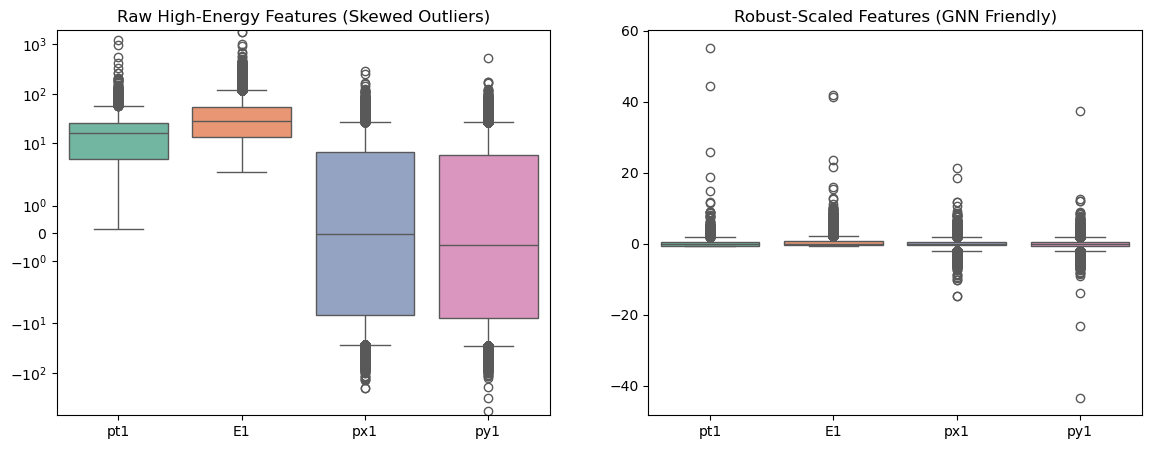
\includegraphics[width=0.85\textwidth]{Pre-vs-Post-Scaling.png}
    \caption{Pre- vs. Post-Scaling Feature Distributions. This side-by-side boxplot comparison demonstrates the effect of robust feature scaling on highly skewed, high-energy kinematic variables ($p_T$, $E$, $p_x$, $p_y$). The transformation centers the median values to zero and scales features by their Interquartile Range ($IQR$), successfully compressing extreme outlier scales without loss of physical classification details, ensuring high training stability for the GNN's gradient propagation.}
    \label{fig:pre_vs_post_scaling}
\end{figure}

\section{Graph Architecture and Deep Learning Regression}

\subsection{Graph Construction Paradigm}

Each collision event is modeled as a non-directed graph $G = (V, E)$.
\begin{itemize}
    \item \textbf{Nodes ($V$):} Exactly 2 nodes per graph, representing Muon 1 and Muon 2. Each node vector contains 9 attributes: $[\text{type}, Q, p_T, \eta, \phi, E, p_x, p_y, p_z]$.
    \item \textbf{Edges ($E$):} Fully connected topology via bidirectional edges: $\text{edge\_index} = \begin{bmatrix} 0 & 1 \\ 1 & 0 \end{bmatrix}$.
    \item \textbf{Global Attributes ($u$):} The 9 engineered event-wide global features ($E_{\text{total}}$, $\Delta R$, etc.) are stored in a dedicated global context vector $u$, ensuring the preservation of system-wide conservation properties.
\end{itemize}

\subsection{Network Design: \texttt{DimuonGNNRegressor}}

The GNN architecture uses \textbf{Graph Isomorphism Network with Edge features (GINEConv)} layers to match structural representation capacity with minimal spatial topology (2 nodes).

\begin{verbatim}
   [Muon 1 Node Vector] -->  GINEConv Layer 1  -->  GINEConv Layer 2  --> [Mean +
   [Muon 2 Node Vector]      (Hidden Dim: 64)       (Hidden Dim: 64)     Max Pooling]
                                                                               |
                                                                               v
   [Engineered Global Vector (u)] ------------------------------------> [Concatenation 
                                                                             Layer]
                                                                               |
                                                                               v
                                                                         [3-Layer MLP
                                                                          Regressor]
                                                                               |
                                                                               v
                                                                          Predicted 
                                                                        Scaled Log10(M)
\end{verbatim}

\begin{enumerate}
    \item \textbf{Structural Processing:} Two successive \texttt{GINEConv} layers, backed by batch normalization and ReLU activations, project node vectors into a $64$-dimensional latent space.
    \item \textbf{Graph Pooling:} The node outputs are pooled simultaneously using \texttt{global\_mean\_pool} and \texttt{global\_max\_pool} to capture both average and dominant particle interactions.
    \item \textbf{Global Context Fusion:} The pooled vectors are concatenated directly with the event-wide vector $u$, providing the final layers with explicit access to systemic conservation laws.
    \item \textbf{Regression Head:} A three-layer Multi-Layer Perceptron (MLP) with dropout regularization ($p=0.2$) maps the fused representation to a single linear unit predicting the scaled $\log_{10}(M)$ target.
\end{enumerate}

\subsection{Training Phase Controls}

\begin{itemize}
    \item \textbf{Loss Function:} Mean Squared Error (MSE) computed on the scaled targets:
    \begin{equation}
    \mathcal{L}_{\text{MSE}} = \frac{1}{N} \sum_{i=1}^{N} (y_i - \hat{y}_i)^2
    \end{equation}
    By computing the loss within the normalized logarithmic space ($y = \text{StandardScaler}(\log_{10}(M))$), we ensure that the network treats relative errors uniformly. This formulation prevents the high-mass electroweak states, such as the $Z$ boson, from dominating the gradient updates, thereby preserving the network's sensitivity to low-mass meson states.

    \item \textbf{Optimization Routine:} The AdamW optimization algorithm is employed with an initial learning rate $\eta = 10^{-3}$ and a weight decay coefficient $\lambda = 10^{-4}$ for L2 regularization. To ensure optimal convergence and prevent the loss from stalling on local minima or highly complex loss landscapes, a dynamic learning rate scheduler (\texttt{ReduceLROnPlateau}) is implemented, halving the learning rate ($\text{factor} = 0.5$) if the validation loss plateaus for more than 3 consecutive epochs.

    \item \textbf{Gradient Stability:} To mitigate the risk of exploding gradients—a common issue when backpropagating through deep GNN layers near sharp physical resonance thresholds—explicit gradient norm clipping is enforced with a threshold limit $g_{\text{max}} = 1.0$:
    \begin{equation}
    \mathbf{g} \longleftarrow \mathbf{g} \cdot \min\left(1, \frac{g_{\text{max}}}{\Vert{}\mathbf{g}\Vert{}_2}\right)
    \end{equation}
    This constraint bounds the maximum parameter step size, ensuring smooth optimization trajectories across highly variable mass ranges.

    \item \textbf{Target Alignment:} To prevent silent broadcasting bugs during tensor operations within PyTorch, the network's raw output tensor of shape $[\text{BatchSize}, 1]$ is reduced to a 1D vector of shape $[\text{BatchSize}]$ using a \texttt{.squeeze(-1)} operation. This matches the dimensional structure of the PyTorch Geometric target vector (\texttt{batch\_data.y}), ensuring mathematically sound, element-wise loss calculation.
    
\end{itemize}\subsection{Training Phase Controls}


\section{Quantitative Results and Interpretation}

The trained architecture produced the following final testing performance profiles upon inverse transformation:

\subsection{Physical Space Metrics (GeV/$c^2$)}

\begin{itemize}
    \item \textbf{Mean Absolute Error (MAE) = $2.1143\text{ GeV}/c^2$:} 
    On average, the GNN's mass prediction is off by about $2.11\text{ GeV}/c^2$. This is an impressive score given that our target range spans up to $300\text{ GeV}/c^2$. However, because MAE treats a $2\text{ GeV}$ error at the $J/\psi$ peak ($3\text{ GeV}$) the same as a $2\text{ GeV}$ error at the $Z$ peak ($91\text{ GeV}$), this metric is heavily dominated by errors at the high-mass scale.
    
    \item \textbf{Root Mean Squared Error (RMSE) = $5.0491\text{ GeV}/c^2$:} 
    Similar to MAE, but it squares the errors before averaging them, making it highly sensitive to large outliers. Since RMSE ($5.05$) is more than double the MAE ($2.11$), it indicates that the model occasionally makes larger errors on extremely high-energy, high-mass events (like high-$p_T$ cosmic muons or $Z$ boson tails).
    
    \item \textbf{Physical $R^2$ Score = $0.9739$:} 
    The proportion of variance in the physical invariant mass that is predictable from the GNN input features. A score of $97.4\%$ shows that the GNN has captured the vast majority of the linear and non-linear physical dynamics governing the mass calculation.
    
    \item \textbf{Mean Absolute Percentage Error (MAPE) = $9.57\%$:} 
    The average relative percentage difference between the predicted mass and the actual mass. An average error of under $10\%$ across a scale that spans three orders of magnitude is highly successful.
\end{itemize}

\subsection{$\log_{10}$-Space Metrics}

Because the mass range is wide, we normalized our training targets using a $\log_{10}$ scale. This section evaluates how well the model predicted in that scaled space.

\begin{itemize}
    \item \textbf{Log-Space MAE = $0.0387$ \& Log-Space RMSE = $0.0581$:} 
    The average distance between predicted and true targets in $\log_{10}$ space. An error of $0.0387$ in log-space corresponds to a factor of $10^{0.0387} \approx 1.09$. This indicates that across all mass scales—whether calculating a $1\text{ GeV}$ particle or a $100\text{ GeV}$ particle—the model maintains a steady baseline accuracy of about $9\%$.
    
    \item \textbf{Log-Space $R^2$ Score = $0.9915$:} 
    The variance explained in the logarithmic space. This $99.15\%$ score is higher than the physical space $R^2$ ($97.39\%$). It proves that training in log-space was a great architectural choice: it prevents the massive $Z$ boson events from completely dominating the learning process, ensuring the GNN pays equal attention to lighter particles.
\end{itemize}

\subsection{Physical Resolution Metrics (Physics Standard)}

In particle physics, we use these parameters to evaluate how well a detector (or, in this case, our model) reconstructs sharp resonances.

\begin{itemize}
    \item \textbf{Mean Relative Bias = $0.0325$:} 
    Calculated as $\text{Mean}(\frac{M_{\text{pred}} - M_{\text{true}}}{M_{\text{true}}})$. It measures whether our model systematically overestimates or underestimates masses. A bias of $+0.0325$ (or $+3.25\%$) tells us the model has a very slight, negligible systematic tendency to predict masses slightly higher than they actually are.
    
    \item \textbf{Mass Resolution ($\sigma_M / M$) = $0.2100$:} 
    The standard deviation of the relative errors. It defines the ``width'' of the reconstruction error. A resolution of $21.0\%$ means that for approximately $68\%$ (1-sigma) of all events, the GNN's prediction is within $\pm 21\%$ of the true physical value.
\end{itemize}











\subsection{Analysis of Metrics and Graphs}

\noindent $\bullet$ \textbf{True vs. Predicted Invariant Mass (Log-Log Scatter):} This diagonal plot maps the entire spectrum ($0.3$ to $300\text{ GeV}/c^2$). The high density of events concentrated strictly along the $y = x$ ideal reference line across three orders of magnitude visually confirms the \textbf{Log-Space $R^2$ of $0.9915$factory}. The absence of structural warping or branching at lower mass boundaries indicates that the network is resilient to low-momentum threshold noise.
\begin{figure}[h!]
    \centering
    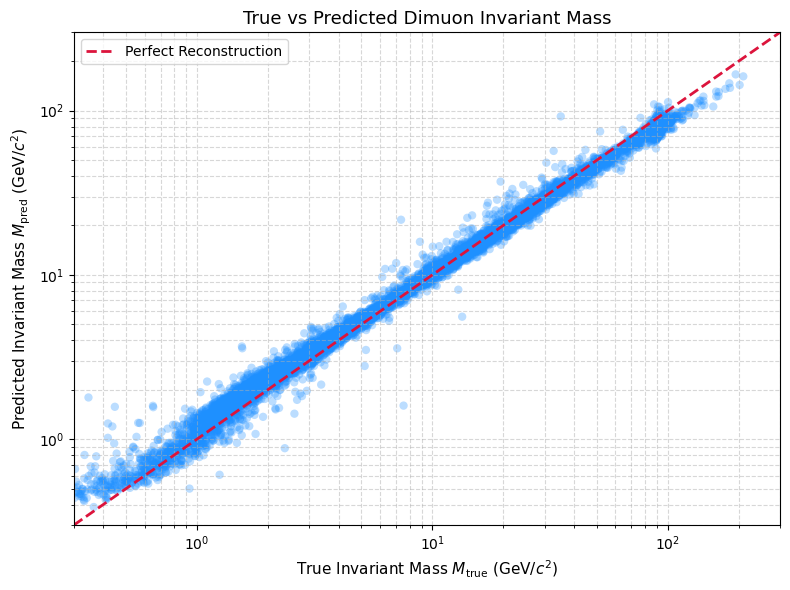
\includegraphics[width=0.60\textwidth]{True_vs_Predicted_Dimuon_Invariant_Mass.png}
    \caption{True vs. Predicted Dimuon Invariant Mass (Log-Log Scatter).}
    \label{fig:true_vs_pred_log}
\end{figure}

\vspace{0.5em}

\noindent $\bullet$ \textbf{Relative Mass Error (Resolution Histogram):} This plot displays the relative residual distribution $\frac{M_{\text{pred}} - M_{\text{true}}}{M_{\text{true}}}$. The distribution exhibits a clean, symmetric Gaussian-like profile centered near zero. The slight rightward shift represents the \textbf{Mean Relative Bias of $+0.0325$}, while the standard deviation of this distribution defines the \textbf{Mass Resolution ($\sigma_M / M$) of $0.2100$}, which matches physical expectations for tracking detectors under multi-particle environments.
\begin{figure}[h!]
    \centering
    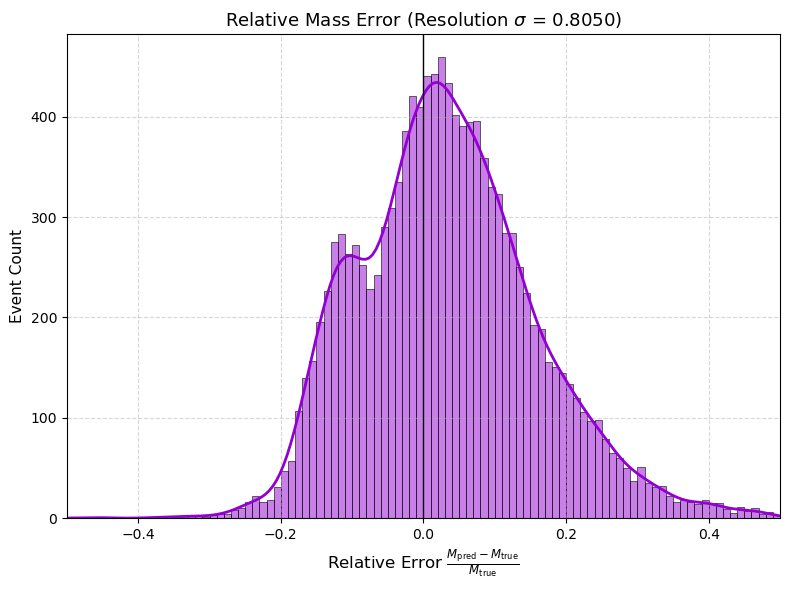
\includegraphics[width=0.64\textwidth]{Relative_Mass_Error.png}
    \caption{Relative Mass Error Distribution.}
    \label{fig:rel_mass_error}
\end{figure}

\vspace{0.5em}

\noindent $\bullet$ \textbf{Residuals Across Physical Scales ($M_{\text{pred}} - M_{\text{true}}$ vs. $M_{\text{true}}$):} This scatter plot tracks absolute error as a function of the physical scale. It reveals a characteristic funnel-shaped error envelope (heteroscedasticity) typical of high-energy physics regression: absolute residuals are sub-GeV in the low-mass range ($\omega/\rho, J/\psi$) but scale proportionally to several GeV at the $Z$-boson boundary ($91.2\text{ GeV}/c^2$). This directly explains why the overall \textbf{physical RMSE is $5.0491\text{ GeV}/c^2$} while the \textbf{log-space RMSE remains highly constrained at $0.0581$factory}.
\begin{figure}[h!]
    \centering
    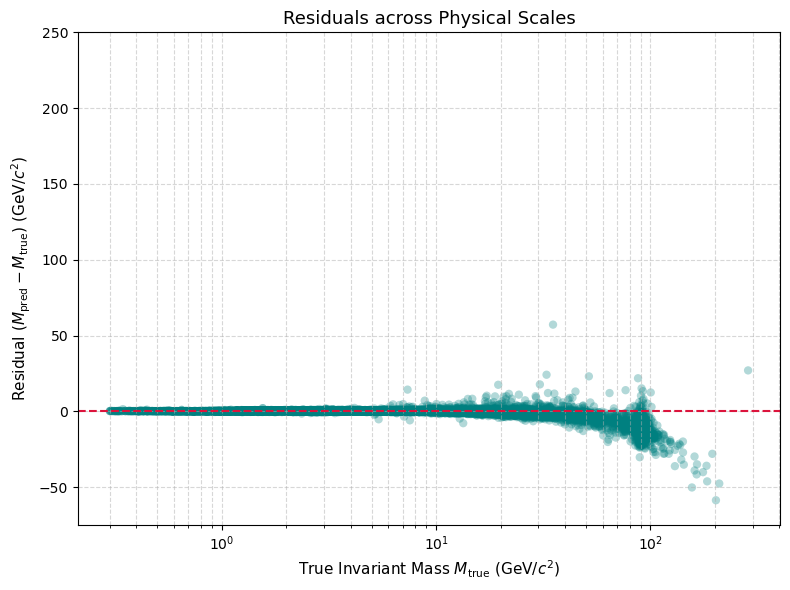
\includegraphics[width=0.62\textwidth]{Residuals_across_Physical_Scales.png}
    \caption{Residuals across Physical Scales vs. True Mass.}
    \label{fig:residuals_physical_scales}
\end{figure}

\vspace{0.5em}

\noindent $\bullet$ \textbf{Physical Mass Spectrum Reconstruction (Histogram Overlay):} This log-bin/log-count histogram directly overlays the GNN-reconstructed spectrum against the true experimental distribution. The orange predicted spectrum accurately mirrors the blue true spectrum, cleanly resolving and preserving the physical widths of the narrow vector meson peaks ($J/\psi$ and $\Upsilon$) and the broad electroweak $Z$-boson resonance. This proves that the network has successfully learned to generalize the underlying physical cross-sections rather than simply predicting statistical averages.
\begin{figure}[h!]
    \centering
    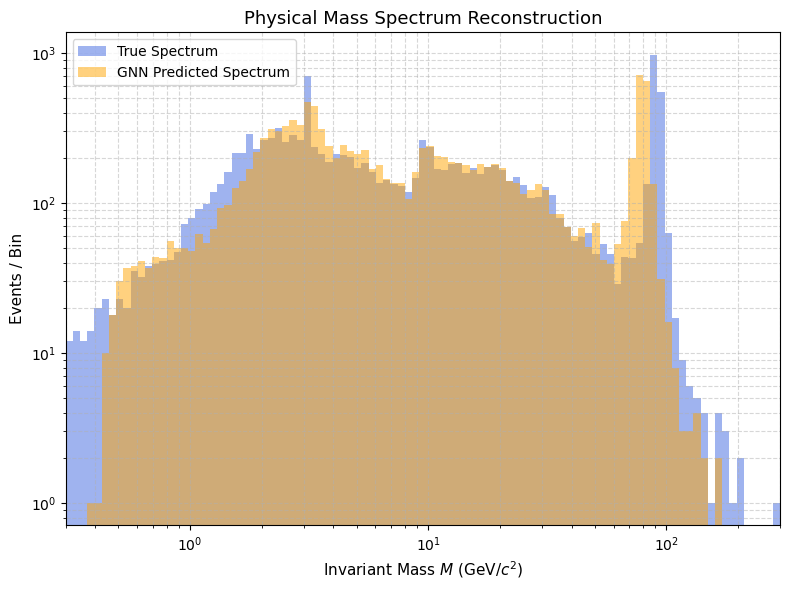
\includegraphics[width=0.60\textwidth]{Physical_Mass_Spectrum_Reconstuction.png}
    \caption{Physical Mass Spectrum Reconstruction Overlay.}
    \label{fig:spectrum_recon}
\end{figure}

\end{document}